\documentclass{ctexart}
\usepackage{multicol}
\usepackage{amsmath, amsfonts, amssymb}
\usepackage{tikz}
\usepackage{geometry}
\special{dvipdfmx:config z 0} % delete this when release

\usetikzlibrary{positioning}

\geometry{a4paper,scale=0.8}

\title{集合论与图论~作业4-6}
\author{庄嘉毅}
\date{September 2022}

\def\QED{\hfill $\square$}
\def\st{\textrm{s.t.}\,}
\def\pair#1{\left\langle #1 \right\rangle}
\def\conj{\mathrel{\wedge}}
\def\disj{\mathrel{\vee}}
\def\equ{\mathrel{\Leftrightarrow}}
\def\restr{\mathbin{\upharpoonright}}
\DeclareMathOperator{\dom}{dom}
\DeclareMathOperator{\ran}{ran}
\DeclareMathOperator{\fld}{fld}
\DeclareMathOperator{\e}{e}

\everymath{\displaystyle}
\linespread{2}

\begin{document}

\maketitle

\section*{习题二}

\paragraph*{6} 证明:

\subparagraph*{(1)} 任取 $\pair{a,c}\in A\times C$,
有 $a\in A \conj c\in C$, 因此 $a\in A\cup B \conj c\in C \cup D$,
故 $\pair(a,c)\in (A\cup B)\times (C\cup D)$, 所以
$A\times C \subseteq (A\cup B)\times (C\cup D)$, 同理
$B\times D \subseteq (A\cup B)\times (C\cup D)$, 故
$(A\times C) \cup (B\times D) \subseteq (A\cup B)\times (C\cup D)$.
\QED

\subparagraph*{(2)} 任取 $\pair{a,c} \in (A-B)\times(C-D)$, 有
$a\in A \conj a\notin B$ 以及 $c\in C \conj c\notin D$, 故
$\pair{a,c} \in A\times C$ 且 $\pair{a,c} \notin B\times D$, 所以
$\pair{a,c} \in (A\times C)-(B\times D)$, 因此
$(A-B)\times(C-D) \subseteq (A\times C)-(B\times D)$.
\QED

\paragraph*{7} 证明:

\subparagraph*{(1)} 对任意 $a, c$, 有
\begin{align*}
    \pair{a,c}\in (A-B)\times C & \equ a \in A \conj a\notin B \conj c\in C                      \\
                                & \equ (a \in A \conj c\in C) \conj (a\notin B \conj c\in C)     \\
                                & \equ \pair{a,c} \in A\times C \conj \pair{a,c}\notin B\times C \\
                                & \equ \pair{a,c} \in (A\times C)-(B\times C)
\end{align*}

故 $(A-B)\times C = (A\times C)-(B\times C)$. \QED

\subparagraph*{(2)}
\begin{align*}
    (A\oplus B)\times C & = ((A-B)\cup (B-A))\times C                       \\
                        & = ((A-B)\times C) \cup ((B-A)\times C)            \\
                        & = (A\times C-B\times C)\cup (B\times C-A\times C) \\
                        & = (A\times C)\oplus(B\times C)
\end{align*}
\QED

\paragraph*{11} 设 $R_1=\{\pair{a,b}, \pair{b,d},\pair{c,c}, \pair{c,d}\}$,
$R_2=\{\pair{a,c}, \pair{b,d},\pair{d,b}, \pair{d,d}\}$, $A=\{a,c\}$.

\subparagraph*{(1)} $R_1\cup R_2=\{\pair{a,b}, \pair{b,d}, \pair{c,c}, \pair{c,d}, \pair{a,c}, \pair{d,b}, \pair{d,d}\}$,

$R_1\cap R_2=\{\pair{b,d}\}$,

$R_1\oplus R_2 = (R_1\cup R_2) - (R_1\cap R_2) = \{\pair{a,b}, \pair{c,c}, \pair{c,d},\pair{a,c}, \pair{d,b}, \pair{d,d}\}$;

\subparagraph*{(2)} $\dom R_1 = \{a,b,c\}$,
$\dom R_2 = \{a,b,d\}$,
$\dom (R_1\cup R_2) = \{a,b,c,d\}$;

\subparagraph*{(3)} $\ran R_1 = \{b,c,d\}$,
$\ran R_2 = \{b,c,d\}$,
$\ran R_1 \cap \ran R_2 = \{b,c,d\}$;

\subparagraph*{(4)} $R_1\restr A = \{\pair{a,b}, \pair{c,c}, \pair{c,d}\}$,
$R_1\restr \{c\} = \{\pair{c,c}, \pair{c,d}\}$,

$(R_1\cup R_2)\restr A = \{\pair{a,b}, \pair{c,c}, \pair{c,d}, \pair{a,c}, \pair{d,b}\}$,

$R_2\restr A = \{\pair{a,c}\}$;

\subparagraph*{(5)} $R_1[A] = \{b,c,d\}$,
$R_2[A] = \{c\}$,
$(R_1\cap R_2)[A]=\{c\}$;

\subparagraph*{(6)} $R_1\circ R_2=\{\pair{a,c}, \pair{a,d}, \pair{d,d}\}$,
$R_2\circ R_1=\{\pair{a,d},\pair{b,b},\pair{b,d},\pair{c,b},\pair{c,d}\}$,

$R_1\circ R_1=\{\pair{a,d},\pair{c,d}, \pair{c,d}\}$.

\paragraph*{12} 设 $R=\{\pair{\varnothing, \{\varnothing, \{\varnothing\}\}}, \pair{\{\varnothing\},\varnothing}, \pair{\varnothing, \varnothing}\}$,

\subparagraph*{(1)} $R^{-1} = \{\pair{\{\varnothing, \{\varnothing\}\}, \varnothing}, \pair{\varnothing,\{\varnothing\}}, \pair{\varnothing, \varnothing}\}$;

\subparagraph*{(2)} $R\circ R = \{\pair{\{\varnothing\}, \{\varnothing, \{\varnothing\}\}}, \pair{\{\varnothing\}, \varnothing }, \pair{\varnothing, \{\varnothing, \{\varnothing\}\}}, \pair{\varnothing, \varnothing}\}$;

\subparagraph*{(3)} $R\restr \varnothing = \varnothing$,
$R\restr \{\varnothing\} = \{\pair{\varnothing, \{\varnothing, \{\varnothing\}\}}, \pair{\varnothing, \varnothing}\}$,
$R\restr \{\{\varnothing\}\} = \{\pair{\{\varnothing\},\varnothing}\}$,

$R\restr \{\varnothing, \{\varnothing\}\} = \{\pair{\varnothing, \{\varnothing, \{\varnothing\}\}}, \pair{\{\varnothing\},\varnothing}, \pair{\varnothing, \varnothing}\}$;

\subparagraph*{(4)} $R[\varnothing] = \varnothing$,
$R[\{\varnothing\}] = \{\{\varnothing, \{\varnothing\}\}, \varnothing\}$,
$R[\{\{\varnothing\}\}] = \{\varnothing\}$,

$R[\{\varnothing, \{\varnothing\}\}] = \{\{\varnothing, \{\varnothing\}\}, \varnothing\}$;

\subparagraph*{(5)} $\dom R = \{\varnothing, \{\varnothing\}\}$,
$\ran R = \{\{\varnothing, \{\varnothing\}\}, \varnothing\}$,
$\fld R = \{\{\varnothing, \{\varnothing\}\}, \varnothing, \{\varnothing\}\}$;

\paragraph*{16}

\subparagraph*{(1)} $R=\{\pair{0,10}, \pair{1,9}, \pair{2,8}, \pair{3,7}, \pair{4,6}, \pair{5,5}, \pair{6,4}, \pair{7,3}, \pair{8,2}, \pair{9,1}, \pair{10,0}\}$,

$S = \{\pair{0,4}, \pair{3,3}, \pair{6,2}, \pair{9,1}\}$;

\subparagraph*{(2)} $R$ 与 $S$ 均不是自反的.

$R$ 不是反自反的, $S$ 是反自反的.

$R$ 是对称的, $S$ 不是对称的.

$R$ 不是反对称的, $S$ 是反对称的.

$R$ 不是传递的, $S$ 是传递的.

\paragraph*{17}
\begin{equation*}
    M(R) = \begin{bmatrix}
        1 & 1 & 1 & 1 \\
        1 & 1 & 1 & 0 \\
        1 & 1 & 1 & 0 \\
        1 & 0 & 0 & 1
    \end{bmatrix}
\end{equation*}

关系图 $G(R)$ 为

\begin{center}
    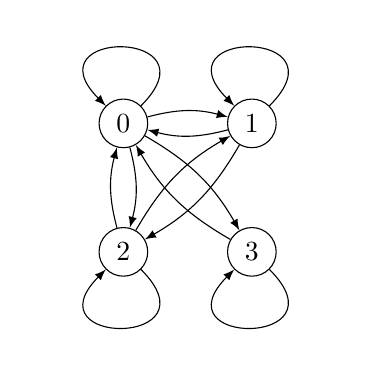
\begin{tikzpicture}
        \node [circle, draw] (0) {0};
        \node [circle, draw, right=of 0] (1) {1};
        \node [circle, draw, below=of 0] (2) {2};
        \node [circle, draw, below=of 1] (3) {3};
        \draw [-latex, in=135, out=45, loop] (0) to ();
        \draw [-latex, in=135, out=45, loop] (1) to ();
        \draw [-latex, in=-135, out=-45, loop] (2) to ();
        \draw [-latex, in=-135, out=-45, loop] (3) to ();
        \draw [-latex, bend left=15] (0) to (1);
        \draw [-latex, bend left=15] (0) to (2);
        \draw [-latex, bend left=15] (0) to (3);
        \draw [-latex, bend left=15] (1) to (0);
        \draw [-latex, bend left=15] (2) to (0);
        \draw [-latex, bend left=15] (3) to (0);
        \draw [-latex, bend left=15] (1) to (2);
        \draw [-latex, bend left=15] (2) to (1);
    \end{tikzpicture}
\end{center}

$R$ 是自反的, 对称的, 不是传递的.

\paragraph*{22} 证明: 由 $R$ 是传递的, 知 $R\circ R\subseteq R$.
任取 $\pair{a,b}\in R$, 由 $R$ 是自反的, 知 $\pair{a,a}\in R$,
故 $\pair{a,b}\in R\circ R$, 因此 $R\subseteq R\circ R$, 故
$R=R\circ R$. \QED

考虑 $R$ 是空关系的情况, 此时满足 $R\circ R=R$, 但由 $A$ 非空, $R$ 不是自反的.

\paragraph*{27} 证明: 记 $M(R_1 \restr \fld R_1) = M_1$,
$M(R_2 \restr \fld R_2) = M_2$, 由 $\fld M_1 \cap \fld M_2=\varnothing$,
知 $M(R_1\cup R_2)=\begin{bmatrix}M_1 & 0 & 0\\ 0 & M_2 & 0 \\ 0 & 0 & 0\end{bmatrix}$,
因此 $M\left((R_1\cup R_2)^m\right)=\begin{bmatrix}M_1^m & 0 & 0\\ 0 & M_2^m & 0 \\ 0 & 0 & 0\end{bmatrix}=M(R_1^m \cup M_2^m)$,
故 $(R_1\cup R_2)^m=R_1^m\cup R_2^m$.

\QED



% 29,35,39,47,50,52

\end{document}
